\section{\tool Overview}
\label{sec:ex}
%$w^Tx>0$, mnist logistic regression
\divya{add reference to before and later... as mentioned we would run evaluations on secure prediction of different models. Here we describe scenario in detail..}

\begin{figure}
  %\vspace{-20pt}
  %\begin{center}
  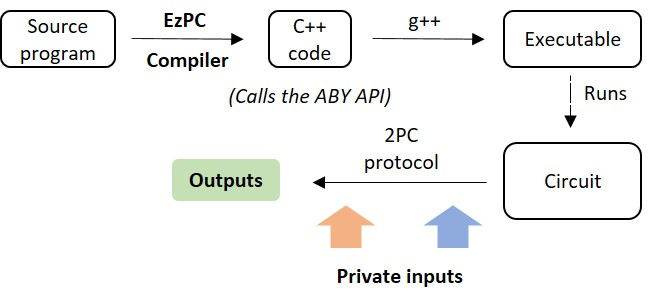
\includegraphics[width=0.45\textwidth]{toolchain}
  %\end{center}
  %\vspace{-20pt}
\caption{\tool toolchain}
\label{fig:toolchain}
\end{figure}



Consider a  cloud service provider Bob that wants to provide a service to diagnose
whether a patient has breast cancer or not. Bob trains a machine learning classification model
that results in a vector $w$ (say of length 30) and a scalar $b$.
This model is the intellectual property of Bob and he  wants to keep it secret.
Given a patient's medical report, in the form of a vector $x$ (also of length 30),
the classifer predicts that the patient has breast cancer if $w^Tx>b$.
However, for this task Bob needs access to $x$, which is private data of a customer.

A potential customer Alice might not want to reveal $x$ to Bob because of privacy concerns.
And Bob does not want to reveal $w$ and $b$ because then Alice can steal the model. \divya{Use HIPAA compliance; as it can leak information of patients that was used in training; more compelling argument. See Shafi intro.}
SMC can help Alice and Bob compute $w^Tx>b$ securely, such that Alice receives the classifier's
prediction and Bob learns nothing about $x$. Moreover, Alice does not learn anything more about $w$
and $b$ than what is revealed by the prediction. 
\nc{This is a bit repetitive from the intro, isnt it? Should we have another example perhaps?}
To implement this system, Bob can write the code in \tool and this code is shown in Figure~\ref{fig:ex-sml}.
The expression {\tt input1} reads a value from Bob and {\tt input2} reads from Alice.
The language has arrays and simple loops. A loop {\tt for i = [0:N]} repeats its
body {\tt N} times, the loop counter {\tt i} is assigned {\tt 0} in the first iteration,
and is incremented by one after each iteration. Unbounded {\tt while} loops are problematic
from a cryptographic standpoint and our language only permits these simple {\tt for} loops. 
The first loop in Figure~\ref{fig:ex-sml} reads the model $w$ from Bob, the second loop reads
Alice's medical report $x$, and the third loop computes the dot product $w^Tx$.
The last {\tt output} statement sends the result of the comparison $w^Tx>b$ to Alice.
In particular, the ternary ``{\tt ? :}" operator performs a branch and the result is the second (third)
argument if the first argument is true (false).

The \tool compiler is fully automatic and compiles the code described in Figure~\ref{fig:ex-sml} to the C++ code that makes calls to the ABY library  in
Figure~\ref{fig:ex-aby}. An alternative to using \tool is to directly write this C++ code.
However, this code is much more complex than the implementation written in \tool.
Therefore, it is difficult for Alice and bob to verify its correctness and security.
Unlike \tool implementations, the ``secret" variables containing private data ({\tt w,x,b,acc}) need to be handled differently compared to ``public" variables such as loop counters ({\tt i}). In particular, the former are manipulated by the ABY library and the latter are manipulated like standard  C++ variables.
Additionally, the C++ code branches on  the special variable
{\tt role}  to decide whether the enclosing code is executed by the {\tt SERVER} Bob or by
the {\tt CLIENT} Alice. In Figure~\ref{fig:ex-sml}, the developer does not need to
manipulate {\tt role} explicitly. In addition to simplifying the implementation, \tool prevents developers from writing buggy code such as\\
\verb+if(role == SERVER) {...manipulate x...}+

Furthermore, the code in Figure~\ref{fig:ex-aby} is too low level.
In particular, it is first builds a circuit that represents the computation
$w^Tx>b$ and then executes it via a call to {\tt ExecCircuit}.
To build a circuit, the code adds multiplication gates ({\tt PutMULGate})
and addition gates ({\tt PutADDGate}) for the dot product.
Subsequently, it uses a ``greater than" gate ({\tt PutGTGate})
and a multiplexer gate ({\tt PutMUXGate}) for the comparison with $b$.
For efficiency, the operations for dot product need to be performed using 
arithmetic circuits. However, ABY's arithmetic circuits cannot express
comparisons and these need  boolean circuits.
A program that uses both arithmetic circuit and boolean circuits
requires conversion gates that help  interconvert between arithmetic
representations and boolean representations ({\tt PutA2YGate}).
Bigger computations often require multiple conversions and the
developer effort can quickly become significant.

Moreover, it is difficult to maintain the code in Figure~\ref{fig:ex-aby}.
For example, if the multiplication is changed to a bitwise-or then,
in the absence of \tool, an efficiency-conscious developer would need to  use boolean circuits everywhere and would be tasked with removing all arithmetic circuits and the interconversion gates (the cost of  conversion overweighs the gains of performing an arithmetic addition instead of a boolean addition). 
 With \tool, the developer needs to change only a single character (replace {\tt *} in Figure~\ref{fig:ex-sml} with {\tt |}) to achieve the same effect. 
On this example and other small examples, we have found that the compiler generated C++ code from a \tool implementation is as efficient as manually written C++ code. In particular, for $w^Tx>b$, the compiler automatically generates code that uses arithmetic circuits for dot product and inserts appropriate conversion gates. Finally, although this paper uses ABY for evaluation, the  compiler can be easily retargeted to generate code for other cryptography backends.


The \tool compiler provides strong static guarantees. For example, a well typed
\tool program is guaranteed to execute to termination without errors. A \tool program cannot go into non-termination or dereference illegal memory, i.e., no buffer overflows or underflows can happen at run time. Production compilers such as {\tt gcc} provide no such guarantees
for the code in Figure~\ref{fig:ex-aby}.
The primary reason that we are able to achieve these guarantees is because
\tool has been designed to be verifiable and is backed by formal semantics. 
Furthermore, the compiler output is guaranteed to be a cryptographically secure
implementation of the functionality declared by the \tool code. 
Moreover, the \tool compiler also generates a C implementation that can be run natively on a single machine for functional testing. 

To summarize, \tool raises the level of abstraction, provides strong static guarantees, and generates efficient code automatically.
